\chapter{Data analysis}
\label{chap:DataAnalysis}
This chapter will engage in the analysis of the acquired flight data from Google Flights. The first part will describe the obtained data. Furthermore, it will describe the cleaning process of the observations, as well as the oulier analysis. The second part will focus on the descriptive analysis of the datasets.

\section{Data description and cleansing}
Flight ticket prices were collected for a period of 42~days ranging from the $9^{th}$ of July till the $29^{th}$ of September. During this data collection phase, airfares on the 22~routes described in \autoref{app:SelectedRoutes} were gathered on flights departing from the $20^{th}$ of August till the $30^{th}$ of September. In these 12~weeks, 158,410~files were requested from Google~Flights' RPC-servers, which resulted in a set of almost 18~gigabytes of JSON~data. Fifteen of these requests failed at the first try, and had to be downloaded again one quarter of an hour later. Of these retries, the automated script also failed to download 2~files at the second request. These failures were the request made on the $20^{th}$ of September at 00:00 GMT+2 for flights departing from JFK to LHR on the $25^{th}$ of September and the request made on the $26^{th}$ of July at 00:00 GMT+2 for flights departing from LHR to LAX on the $1^{st}$ of July. Due to the methodology applied by this research, in which 4~daily time windows are aggregated into a single value, these 2~failures did not create any gaps of missing values in the final data matrix.

After retrieval of the data all the JSON-files were parsed for airfares of flights. As stated in \autoref{sub:CharacteristicsOfTheFlightTicket}, this research only includes single-legged round~trip flights between the defined 22~routes between outbound and inbound airport. The parsing of the files resulted in a matrix with rows containing a flight's fare history in 6~hour time windows. These windows were then converted into daily observed airfares. The conversion into daily values resulted in a database containing 462,662 unique flights which included 12,865,953 airfare observations. Due to Google Flights' nature of returning a limited set of airfares for each request, some flights did contain gaps of missing values within their data. In alignment with the study by \citeA{groves2013agent}, this paper therefore excludes flights for which less than $\frac{2}{3}$ of the possible airfare observations are available. So, because there are a total of 42~observations days prior to each flight, tickets that do have fewer points than $42 \times \frac{2}{3} = 28$ available will be excluded from the analysis. Next, because airlines are known to open and close specific price-buckets \cite{mcgill1999revenue}, some gaps were still present in the dataset. These gaps were filled with the data available from observations made in the future. For example, when a particular flight misses a price observation at 35~days before departure, but it does contain the airfare for 34 and 36~days prior to departure, the 35~days' window would be filled with the same value as the 34~days before departure. In reality this would mean that when a customer's option expires, but the ticket is not available on the date of maturity (i.e., no price observation). The customer thus would have to wait till the airline resumes the sale of that flight. He would therefore get the ticket at the price in the future.

Missing data at for the last (few) days prior to departure are considered to be the sell-out of a flight. Because Google Flights' also offers Business and First class tickets, this implies that all the seats are completely sold out, and there is no possibility of still buying the ticket. This means that when a customer's option expires on such a ticket and he wishes to exercise it, an alternative flight has to be offered. To prevent such situations from happening, these missing data on sold-out flights is filled with a penalty similar to the technique used by \citeA{etzioni03}. By introducing such a penalty, the option valuation model is triggered into trying not to offer options when the probability of sell-out is high. Instead of the \$300,000 proposed by the authors, I have chosen to set the penalty at 3 times the average airfare at 1~day before departure. This is more realistic in a sense that the customer could be offered an alternative flight that leaves on the same day plus some extra form of monetary compensation. Furthermore this lower fill-value prevents penalties from biasing the airfares closer to departure.

An illustration of this data filling process is given in \autoref{fig:dataFillingOfMissingValues}. Airfares are given as integers representing the price in cents. As can be seen in the figure, the n/a-gaps are filled with the nearest available future price closer to departure. Furthermore, the missing value for the flight with id~\#3 at 1~day before departure is seen as a sold-out ticket. This value is filled with $3 \times \bar{c_1}$, where $\bar{c_1}$ represents the average of the airfares observed at a single day before departure.

\begin{figure}
$$
\kbordermatrix{
           & 1\,\scriptstyle{dbd} & 2\,\scriptstyle{dbd} & 3\,\scriptstyle{dbd}  & \cdots \\
    \#1    & 10000                & 12000                & 12000                 & \cdots \\
    \#2    & 20000                & \mathrm{n/a}         & 22000                 & \cdots \\
    \#3    & \mathrm{n/a}         & 32000                & \mathrm{n/a}          & \cdots \\
    \vdots & \vdots               & \vdots               & \vdots                & \ddots
}
\Rightarrow
\kbordermatrix{
           & 1\,\scriptstyle{dbd} & 2\,\scriptstyle{dbd} & 3\,\scriptstyle{dbd}  & \cdots \\
    \#1    & 10000                & 12000                & 12000                 & \cdots \\
    \#2    & 20000                & 20000                & 22000                 & \cdots \\
    \#3    & 3 \cdot \bar{c_1}    & 32000                & 32000                 & \cdots \\
    \vdots & \vdots               & \vdots               & \vdots                & \ddots
}
$$
\caption{Data filling of missing values (i.e., n/a)}
\label{fig:dataFillingOfMissingValues}
\end{figure}

The empirical dataset shows that in total 15,643 flights are not offered (i.e., sold out) at 1~day before departure. These tickets take into account 5.6 percent of the all the flights available. Real-world data on the number of sold out flights is very hard to acquire, because this value could give sensitive information on the performance of an airline. However, this number of sold outs seems to be on the low side. A possible explanation for this might be that this research only requests airfares up till 1~day before departure. So, likely a higher number of sold outs will be observed when one also requests the fares on the day of departure. Furthermore, due to the time window averaging of the 4~daily fare observations, the daily value actually includes all ticket prices acquired 24~till 48~hours before departure.

After cleaning the dataset, it was split into two separate parts. The database used in this research contains airfare observations of flights departing in the period $20^{th}$ of August till the $30^{th}$ of September. As explained in \autoref{chap:Methodology}, the first 4~weeks of these departing flights --- $20^{th}$ of August till the $16^{th}$ of September --- will be used as the training set for the research. The latter 2~weeks --- from the $17^{th}$ of September till the $30^{th}$ of September --- will be used for testing the proposed option valuation models. This split resulted in a training set containing 321,545 flights, and a test set which includes 141,117 flights. An example extract of the final test data matrix used for the flights from AMS to JFK can be found in \autoref{fig:extractFromAMStoJFK}. In this extract, the flight with id~\#4 was sold-out 1~day before departure, and that field was thus filled with $3 \times$ the average ticket price at 1~day before departure.

\begin{figure}
$$
\kbordermatrix{
           & 1\,dbd & 2\,dbd & 3\,dbd & 4\,dbd & 5\,dbd & \ldots & 42\,dbd \\
    \#1    & 57469  & 68619  & 122469 & 222469 & 109644 & \ldots & 65853   \\
    \#2    & 87119  & 87369  & 93019  & 84469  & 79469  & \ldots & 65853   \\
    \#3    & 87494  & 86694  & 94744  & 74569  & 70244  & \ldots & 65853   \\
    \#4    & 410951 & 134430 & 242480 & 108934 & 126369 & \ldots & 123357  \\
    \vdots & \vdots & \vdots & \vdots & \vdots & \vdots & \ddots & \vdots  \\
    \#252  & 68984  & 69094  & 64669  & 73219  & 70244  & \ldots & 65857
}
$$
\caption{Sample extract from test data matrix AMS to JFK}
\label{fig:extractFromAMStoJFK}
\end{figure}


\subsection{Outlier analysis}
\label{subsec:outlierAnalysis}
After cleansing the dataset, the outlier analysis was performed. First, extreme and invalid prices were identified and removed from the dataset. Google Flights sometimes yielded with an impossible airfare for a flight, and it is more likely that such values were not prices, but rather codes for the website. For example, when Google Flights does currently not have recent price information on a flight, the ticket price was set at 3. This of course is an impossible price for a flight, even more so considering the prices returned are in cents. To exclude these codes from the dataset, all airfares lower than 1,000~cents were removed from the dataset (i.e., $p_i < 1000$).

For the next step of the outlier analysis, box plots of the observed ticket prices were generated. These plots are displayed in \autoref{fig:BoxplotsWithOutlierAnalysis}. The whiskers for these plots have been set to 1.5~times the interquartile range.

A quick analysis of these figures shows that there are many theoretical outliers available for each flight. In this research, however, I have chosen not to exclude these from the actual dataset. The reason for this is that these airfares have been empirically observed, and could therefore appear in a real world setting. These airfares could arise when the seats in the economy~class for that flight were sold out, and the cheapest available option was an upgrade to first or business~class. When these values would be removed from the dataset, a too optimistic view could arise. In such a view the simulated risk would be undervalued and profits would be overestimated. This would lead to a misfit between this research and the real world application, and the results would yield worthless.

Furthermore, as will be demonstrated in \autoref{subsec:DescriptiveAnalysisOfFareChanges}, the strong tendency of the data towards `no price change' could have lead to a underestimated standard deviation. Therefore, the box~plots might label some observations as outliers, while this is actually not the case.

Because of these reasons, I have decided to not exclude these observed outliers from the dataset.


\begin{figure*}
\centering
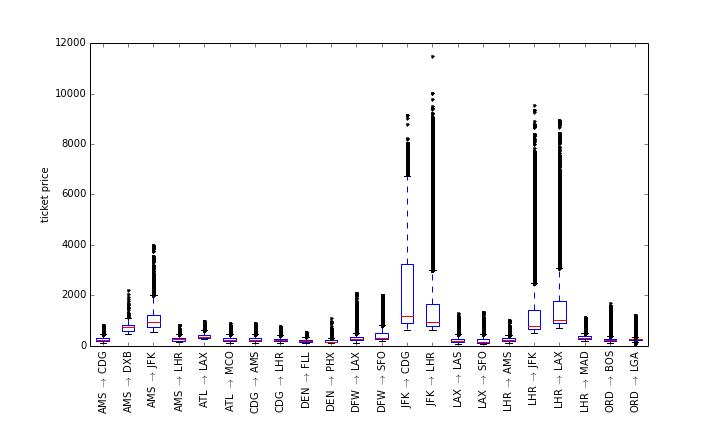
\includegraphics[width=.8\textwidth]{figures/outlierAnalysis}
\caption{Box plots with outlier analysis}
\label{fig:BoxplotsWithOutlierAnalysis}
\end{figure*}


\section{Exploratory data analysis}
In this section the exploratory data analysis is performed on the dataset after cleansing. First, a descriptive analysis is performed on the number of flights, observations and sold outs of both datasets. Next an analysis is performed on the ticket prices and daily price fluctuations. This analysis also includes a test of normality to see whether the distribution follows a log-normal distribution. Lastly, a comparison between the training and the test dataset is made to see whether they differ significantly.

Throughout this research, a distinction is made between two databases, namely: the training and the test dataset. The \emph{training} dataset will be used as historical airfare information on which the customer bases its forecasts. Furthermore, the training dataset is also used by the seller in the Black--Scholes and Monte~Carlo models to compute his Willingness To Accept. The \emph{test} set is used to evaluate the option pricing models.

\subsection{Descriptive analysis of flights}
First, the descriptive analysis on the flights is performed. The results of this analysis on all the flights available in the total dataset, as well as the distinction between test and training, can be found in \autoref{tbl:DescriptiveAnalysisTotalDataset}. The \emph{Flights -- total} row displays the total number of unique flights available in the specified dataset. \emph{Flights -- valid} shows the count of flights that exceed a certain threshold of daily observations made for that route. As stated in \autoref{chap:Methodology}, only flights with more than 28~observations\footnote{Two-thirds of the total 42~possible observations} are included in the analysis. The \emph{Fares -- total} line gives the total number of airfare observations made in the dataset containing only the valid flights. The last two rows specify the number and percentage of sold outs in the data.

As one can deduce from this analysis, the training set is significantly larger than the test data. This is due to the split in empirical data. The first 4~weeks of the set are assigned to the training dataset, while only the latter 2~were selected to be the census for the test set. In a real world application of option valuation models this is likely to be also the case, as there is much more historical data available to the option seller than there are flights on which he has to make forecasts for. The difference in counts in both datasets is not expected to be of influence on the results of the simulation model, as there are a vast amount of data available to both sets.

The costs due to sold outs, however, is expected to be higher due to the difference between both sets. The Black--Scholes and Monte~Carlo models both base their predictions upon the historical (i.e., training) dataset, and will therefore likely expect an equal amount of sold outs of flights in the test set. However, as can be seen from the data, the test dataset contains about 15~percent more sold outs than the training dataset.

\begin{table}
\centering
\footnotesize
\begin{tabular}{l l r r r}
    \toprule
    ~         &  ~          &  Total dataset  & Test dataset  &  Training dataset \\ 
    \midrule
    Flights   &  total      &  462,662    &  141,117    & 321,545 \\
    ~         &  valid      &  278,349    &  98,916     & 179,433 \\
    ~         &  valid (\%) &  60,2       &  70.1       & 55.8 \\
    Fares     &  total      &  11,280,278 &  4,064,937  & 7,215,341 \\
    Sold outs &  total      &  15,643     &  6,053      & 9,590 \\
    ~         &  total (\%) &  5.6        &  6.1        &  5.3 \\
    \bottomrule
\end{tabular}
\caption{Descriptive analysis total dataset}
\label{tbl:DescriptiveAnalysisTotalDataset}
\end{table}


A route-specific descriptive analysis of both datasets can be found in \autoref{tbl:DescriptiveAnalysisTestDataset} and \autoref{tbl:DescriptiveAnalysisTrainingDataset}.


\begin{table}
\centering
\footnotesize
\begin{tabular}{c c | c c c | c | c c}
\toprule
\multicolumn{2}{c|}{Airport}  & \multicolumn{3}{c|}{Flights} & Fares & \multicolumn{2}{c}{Sell outs} \\[.4ex]
from &  to  & total  & valid  & valid (\%)  &  total  &  total  &  total (\%) \\
\midrule
AMS  &  CDG  &   4,630  &   3,936  &   85.0  &  164,706  &    146  &   3.7 \\
~    &  DXB  &      14  &      14  &  100.0  &      588  &      0  &   0.0 \\
~    &  JFK  &     252  &     252  &  100.0  &   10,572  &      6  &   2.4 \\
~    &  LHR  &   2,834  &   2,558  &   90.3  &  106,611  &    108  &   4.2 \\[.5ex]
ATL  &  LAX  &   1,776  &   1,421  &   80.0  &   59,225  &      3  &   0.2 \\
~    &  MCO  &   4,727  &   3,757  &   79.5  &  156,488  &     24  &   0.6 \\[.5ex]
CDG  &  AMS  &   4,149  &   3,936  &   94.9  &  165,125  &     94  &   2.4 \\
~    &  LHR  &   1,264  &   1,250  &   98.9  &   52,437  &     14  &   1.1 \\[.5ex]
DEN  &  FLL  &      21  &      21  &  100.0  &      865  &      4  &  19.0 \\
~    &  PHX  &   1,541  &   1,453  &   94.3  &   60,847  &     50  &   3.4 \\[.5ex]
DFW  &  LAX  &  11,157  &   8,872  &   79.5  &  368,838  &    467  &   5.3 \\
~    &  SFO  &   5,272  &   4,503  &   85.4  &  182,895  &    578  &  12.8 \\[.5ex]
JFK  &  CDG  &   2,569  &   1,782  &   69.4  &   73,119  &    146  &   8.2 \\
~    &  LHR  &  10,824  &   7,918  &   73.2  &  331,646  &    182  &   2.3 \\[.5ex]
LAX  &  LAS  &   7,642  &   5,334  &   69.8  &  208,889  &    431  &   8.1 \\
~    &  SFO  &  32,367  &  16,161  &   49.9  &  653,809  &  1,317  &   8.1 \\[.5ex]
LHR  &  AMS  &   2,788  &   2,567  &   92.1  &  107,431  &     50  &   1.9 \\
~    &  JFK  &   9,981  &   7,690  &   77.0  &  322,109  &    159  &   2.1 \\
~    &  LAX  &   1,581  &     837  &   52.9  &   34,580  &     58  &   6.9 \\
~    &  MAD  &   4,758  &   4,732  &   99.5  &  198,705  &     26  &   0.5 \\[.5ex]
ORD  &  BOS  &   9,037  &   7,204  &   79.7  &  287,993  &  1,140  &  15.8 \\
.    &  LGA  &  21,933  &  12,718  &   58.0  &  517,459  &  1,050  &   8.3 \\
\bottomrule
\end{tabular}
\caption{Descriptive analysis of test dataset}
\label{tbl:DescriptiveAnalysisTestDataset}
\end{table}


\begin{table}
\centering
\footnotesize
\begin{tabular}{c c | c c c | c | c c}
\toprule
\multicolumn{2}{c|}{Airport}  & \multicolumn{3}{c|}{Flights} & Fares & \multicolumn{2}{c}{Sell outs} \\[.4ex]
from &  to  & total  & valid  & valid (\%)  &  total  &  total  &  total (\%) \\
\midrule
AMS  &  CDG  &   8,389  &   7,871  &  93.8  &  329,235  &    136  &   1.7 \\
~    &  DXB  &      35  &      28  &  80.0  &    1,176  &      0  &   0.0 \\
~    &  JFK  &     639  &     638  &  99.8  &   26,796  &      0  &   0.0 \\
~    &  LHR  &   5,380  &   4,891  &  90.9  &  204,906  &    110  &   2.2 \\[.5ex]
ATL  &  LAX  &   3,613  &   3,203  &  88.7  &  133,976  &      8  &   0.2 \\
~    &  MCO  &   8,554  &   7,602  &  88.9  &  317,860  &     39  &   0.5 \\[.5ex]
CDG  &  AMS  &   8,186  &   7,874  &  96.2  &  329,613  &    107  &   1.4 \\
~    &  LHR  &   2,577  &   2,529  &  98.1  &  106,218  &      0  &   0.0 \\[.5ex]
DEN  &  FLL  &      58  &      45  &  77.6  &    1,792  &      6  &  13.3 \\
~    &  PHX  &   2,433  &   2,426  &  99.7  &  101,656  &     89  &   3.7 \\[.5ex]
DFW  &  LAX  &  36,579  &  14,845  &  40.6  &  559,879  &    247  &   1.7 \\
~    &  SFO  &  16,117  &   7,436  &  46.1  &  279,339  &    313  &   4.2 \\[.5ex]
JFK  &  CDG  &   4,947  &   3,238  &  65.5  &  132,385  &    354  &  10.9 \\
~    &  LHR  &  23,440  &  14,825  &  63.2  &  610,280  &  1,489  &  10.0 \\[.5ex]
LAX  &  LAS  &  16,261  &   9,782  &  60.2  &  385,907  &    319  &   3.3 \\
~    &  SFO  &  68,886  &  24,929  &  36.2  &  988,534  &  1,928  &   7.7 \\[.5ex]
LHR  &  AMS  &   5,230  &   4,904  &  93.8  &  204,973  &    193  &   3.9 \\
~    &  JFK  &  22,540  &  14,711  &  65.3  &  606,489  &  1,039  &   7.1 \\
~    &  LAX  &   3,513  &   1,597  &  45.5  &   64,877  &    289  &  18.1 \\
~    &  MAD  &   9,464  &   9,438  &  99.7  &  395,966  &     67  &   0.7 \\[.5ex]
ORD  &  BOS  &  24,145  &  12,904  &  53.4  &  493,077  &  1,624  &  12.6 \\
~    &  LGA  &  50,559  &  23,717  &  46.9  &  940,407  &  1,233  &   5.2 \\
\bottomrule
\end{tabular}
\caption{Descriptive analysis of training dataset}
\label{tbl:DescriptiveAnalysisTrainingDataset}
\end{table}


The number of flights with a valid number of fare observations differs a lot amongst some routes. For example, the route AMS to DXB only has a single observation per data collection day, while a route like LAX to SFO contains almost 25,000~valid flights in the training set. This high difference has to do with the number of single-legged flights available on each route. AMS to DXB offers only a single option every day, which is operated by a single airliner (KLM). Hence, it only returns a single valid round~trip flight for each day. The route between LAX and SFO, however, offers around 50~direct flights operated and ticketed by different carriers. Google Flights computes different possible round~trip flights and returns the fares for these specific configurations. Because each configuration of outbound and inbound flights is considered as a different combination, the number of possible round~trip flights increases significantly.

Another observation that can be made from the tables, is that the percentage of valid flights for a route is significantly lower for routes with a high number of total flights. This also has to do with Google Flights' methodology. As stated in previous paragraph, Google creates its own combinations of round~trip flights, and returns the airfares. When the number of combinations exceeds a certain amount, the website does only return a selection of the fares. As a result, not always the ticket prices for the same set of flights are returned. Because a route with a higher number of combinations is more likely to exceed the threshold of maximum airfares, a request for this route will only return a partial set of prices. This thus creates gaps in the data, which results in less valid flights.

As stated previously, the differences in flights and observations between the training and test dataset will not have any major influences on routes with a fair amount of observations. The two routes with little observations --- AMS to DXB and DEN to FLL --- might therefore give skewed results which might not apply to similar routes.

The differences between the percentage of sold outs, however, is expected to be of influence on the results. Routes with a lower percentage of sold outs in the training set than in the test data are likely to yield lower profits when nearing the departure of a flight. This is due to an underestimated sold out risk, which will lead to higher penalty costs. Flights like the ones departing from AMS are expected to show such behaviour, as these have high relative differences amongst the sets.

When the historical data shows lower sold outs than observed in the test dataset the profits will generally also tend to be lower when nearing the departure date. This is not the result of extra penalty costs, but due to missed sales because of overestimation of the sold out risk. However, in the simulation model used in this thesis, the customer also bases its forecasts on the same historical data. He will therefore also overestimate the expected risk of a sold out, and is willing to pay for this risk. The routes with a higher sell out in the training set than in the test data are therefore expected to generate more profits when closing to the final date. This is expected to particularly expected for flights on the route LHR to LAX, as their sold out rate for the training and test set is 18.1\,\% and 6.9\,\% respectively.


\subsection{Descriptive analysis of fare changes}
\label{subsec:DescriptiveAnalysisOfFareChanges}
This section engages in the descriptive analysis of the fare changes of the ticket prices.

A price change in this research is defined as the daily logarithmic change between $p_t$ and $p_{t+1}$, where $t$ is the number of days before departure (i.e., dbb). This paper uses the definition as seen in \citeA{mun2006real} to calculate the relative changes:

\begin{equation*}
    \begin{split}
    x_t &= \ln(p_{t}) - \ln({p_{t+1}}) \\
    &= \ln\left( \frac{p_{t}}{p_{t+1}}\right) 
    \end{split}
\end{equation*}


The mean, variance, and range of the airfares as well as the price fluctuations are computed on the entire dataset. The results of this analysis are displayed in \autoref{tbl:DescriptiveAnalysisEntireDataset}.

As can be seen in the table, the range for the ticket prices is quite large. The high maximum ticket price can be explained by the fact that Google Flights also returns prices of first and business~class seats. The website normally returns the fares of the lowest available option. However, when regular economy~class tickets are sold out, the Google Flights will yield the next-lowest fare, which could be an available business~class seat. The low minimum ticket prices can be described by the airliners offering cheap fares at the beginning of the booking period, and some high price~drops at 1~day before departure.

The data also shows that the route CDG to JFK has the highest average ticket price, as well as the largest standard deviation. This is because of the unregular spread seen in fares for flights covering this specific route. While in other routes the observed prices were clustered together with only a few exceptions (i.e., outiers), the flights for the route CDG to JFK seemed to have multiple means. For illustration, \autoref{fig:SpreadOfTicketPrices} gives a comparision of ticket price distribution of this specific route, and the example of the spread of flights leaving from AMS to LHR.


\begin{table}
\centering
\footnotesize
\begin{tabular}{c c | c c c c | c c c c}
\toprule
\multicolumn{2}{c|}{Airport}  & \multicolumn{4}{c|}{Ticket price} & \multicolumn{4}{c}{Daily changes} \\[.4ex]
from & to    &  $\mu_{p}$ & $\sigma_{p}$  &  $\min_p$  & $\max_p$  & $\mu_x$ & $\sigma_x$  & $\min_x$  &  $\max_x$ \\ 
\midrule
AMS  &  CDG  &   237  &    79  &    98  &   835  &  0.019  &  0.084  &  -0.968  &  1.009  \\
~    &  DXB  &   718  &   165  &   467  &  2205  &  0.007  &  0.063  &  -0.461  &  0.977  \\
~    &  JFK  &  1023  &   334  &   546  &  3975  &  0.008  &  0.066  &  -0.843  &  1.093  \\
~    &  LHR  &   262  &    81  &   128  &   816  &  0.012  &  0.050  &  -0.603  &  0.673  \\[.5ex]
ATL  &  LAX  &   383  &    60  &   251  &   985  &  0.015  &  0.066  &  -0.674  &  0.651  \\
~    &  MCO  &   239  &    47  &    89  &   900  &  0.021  &  0.079  &  -0.606  &  0.689  \\[.5ex]
CDG  &  AMS  &   245  &    81  &    98  &   915  &  0.018  &  0.078  &  -1.053  &  1.036  \\
~    &  LHR  &   231  &    74  &    97  &   780  &  0.010  &  0.080  &  -1.027  &  0.818  \\[.5ex]
DEN  &  FLL  &   193  &    61  &    89  &   546  &  0.010  &  0.063  &  -0.386  &  0.537  \\
~    &  PHX  &   186  &    45  &   103  &  1101  &  0.014  &  0.065  &  -0.923  &  1.043  \\[.5ex]
DFW  &  LAX  &   312  &    86  &   110  &  2068  &  0.023  &  0.076  &  -1.695  &  1.690  \\
~    &  SFO  &   380  &   124  &   164  &  2018  &  0.023  &  0.095  &  -1.263  &  1.370  \\[.5ex]
JFK  &  CDG  &  2353  &  2177  &   638  &  9164  &  0.012  &  0.083  &  -1.592  &  1.783  \\
~    &  LHR  &  1389  &   959  &   604  &  11498  &  0.024  &  0.131  &  -1.998  &  1.988  \\[.5ex]
LAX  &  LAS  &   205  &    90  &    54  &  1306  &  0.012  &  0.100  &  -1.633  &  1.635  \\
~    &  SFO  &   207  &   112  &    82  &  1332  &  0.020  &  0.106  &  -1.810  &  1.333  \\[.5ex]
LHR  &  AMS  &   255  &    93  &   113  &   996  &  0.013  &  0.050  &  -0.691  &  0.733  \\
~    &  JFK  &  1177  &   831  &   510  &  9565  &  0.012  &  0.118  &  -2.141  &  2.169  \\
~    &  LAX  &  1554  &  1073  &   683  &  8944  &  0.011  &  0.155  &  -1.823  &  2.129  \\
~    &  MAD  &   330  &    90  &   172  &  1141  &  0.010  &  0.057  &  -1.006  &  0.848  \\[.5ex]
ORD  &  BOS  &   245  &    61  &    89  &  1682  &  0.014  &  0.072  &  -1.352  &  1.441  \\
~    &  LGA  &   272  &    49  &    89  &  1219  &  0.014  &  0.063  &  -0.946  &  1.159  \\
\bottomrule
\end{tabular}
\caption{Descriptive analysis of entire dataset}
\label{tbl:DescriptiveAnalysisEntireDataset}
\end{table}


\begin{figure*}
\centering
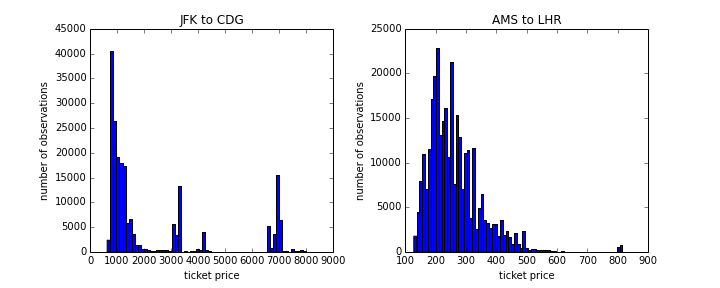
\includegraphics[width=.8\textwidth]{figures/Spread_JFK-CDG}
\caption{Spread of ticket prices}
\label{fig:SpreadOfTicketPrices}
\end{figure*}


The high range observed in the price fluctuations in some cases can also be assigned to sudden fare increases and drops. The high drops appearing at a single day before departure when the flight is yet to be sold out. This as a last resort of the airline to fill the seats on the plane. The high increases can be explained due to sold outs of economy~class tickets, which results in the display of first and business~class tickets.

For a better understanding of the price movements of airfares, one can look at the run sequence plot in \autoref{fig:4-plot}. The chart shows the average and standard deviation of price fluctuations of all the flights in the complete dataset. Instead of categorisation per route, the plot shows the statistics relative to its number of days before departure. One can clearly see that the mean fares for tickets are relatively stable for about the first three weeks of the analysis. The last three weeks up till departure there can clearly be seen significant and increasing price jumps at around 21~days, 14~days, 7~days, and the last few days before the flight. Furthermore, throughout the whole time frame, the volatility of the price fluctuations seems to be increasing.


\begin{figure*}
\centering
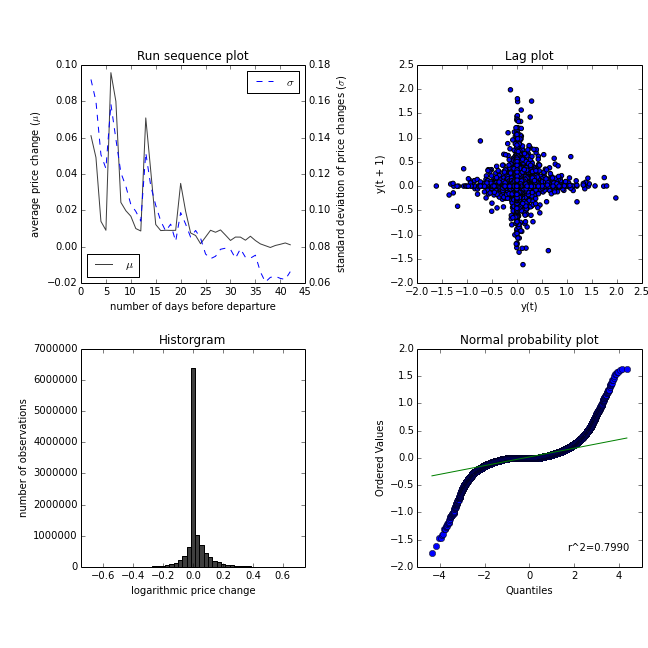
\includegraphics[width=.8\textwidth]{figures/4-plot}
\caption{4-Plot of the daily price fluctuations}
\label{fig:4-plot}
\end{figure*}


Due to these price jumps and increasing volatility, there will be more uncertainty on price fluctuations when nearing the departure date of the flight. Therefore it is expected that the option valuation models will yield higher airfare~lock-in prices for days closer to the flight's take-off. The higher standard deviation also creates more risk, which will likely result in higher losses and lower profits for those options than the ones that are offered at the beginning of the booking period.

The empirical distribution of all the ticket price fluctuations is presented in the histogram of \autoref{fig:4-plot}. The chart seems to display a normal distribution with a very high kurtosis and a strong tendency to the logarithmic price change of 0. The \emph{zero} can be interpreted as `no price change', and accounts for more than 56~percent --- or more than 6~million --- of all observed price changes. Due to this extreme peak, the empirical distribution can not be classified as a normally distributed one.

Analysis of the lag~plot in the same figure also results in the conclusion that the data on price fluctuations is not normally distributed. The plot consists of a random sample of 10,000~price changes, and clearly shows a cross-like figure near the 0-axes. Furthermore, the observations seem to be skewed to the positive quadrant of the figure. Both observations thus imply that the data is not random normally distributed.

The lag~plot also shows some outliers. However, as explained in \typenameref{subsec:outlierAnalysis}, these extreme values will be left included in the simulation models and data analysis. This is because these observations are valid empirical price changes, and could thereby happen in a real world setting.

The last visual confirmation that the data containing airfare fluctuations in not normally distributed can be found in the normal probability plot. This figure evidently shows that the data do not follow a straight line as a normal dataset would. 

The analysis of the 4~plot thus shows that the daily price fluctuations are not normally distributed. This is also confirmed by other normality tests. \autoref{tbl:NormalityTests} shows the results of the Shapiro--Wilk and Kolmogorov--Smirnov test for normality. Furthermore, it also displays the outcome of SciPy's implementation of \emph{normaltest}, which is based upon D'Agostino's K-squared and Pearon's chi-squared test.

All these statistical formula's test the null hypothesis, $H_0$, that the supplied sample came form a normally distributed population. As the outcomes of these tests show in the table, all of the tests lead to rejection of the null hypothesis. It can therefore be concluded that the daily price fluctuations do not follow a normally distributed curve.


\begin{table}
\centering
\begin{tabular}{l c c c}
\toprule
~  &  Test statistic  &  p-value  &  Reject $H_0$  \\
\midrule
Shapiro--Wilk test  &  0.66  &  $< 0.001$  & yes \\
Kolmogorov--Smirnov test  & 0.42  &  $< 0.001$  & yes \\
Normal test  & $6.34 \e{6}$  & $< 0.001$  & yes \\
\bottomrule
\end{tabular}
\caption{Tests for normality of daily returned values}
\label{tbl:NormalitTests}
\end{table}


The non-normality of the data implies that the changes in ticket prices are not completely random, and can therefore be predicted to some extend. Furthermore, because the daily changes are not (log-)normally distributed, the simulation model based upon Black--Scholes is not expected to perform well. This is due to one of the base assumptions of the Black-Scholes model which state that the underlying asset's returns follow a log-normal distribution. The optimal option price predictions according to this model are therefore likely to be far off of the optimal, which will lead to lower profits.

\subsection{Comparison of the training and test dataset}
This section compares the two different datasets with each other. As stated before, the first 4~weeks of data collected are assigned to the training (i.e., historical) dataset, and the last 2~weeks of the collection period to the test dataset. The two practically feasible option valuation methods in this research both use the historical set to make predictions of the price fluctuations in the test set. The Black--Scholes model uses the training dataset to determine the expected volatility of the ticket prices. The Monte~Carlo model bases its forecasts of airfares upon the empirical distribution seen in the same historical dataset. For these reasons, when the datasets differ from each other, the predictions of the models are likely to have a bigger error. The forecasts of the ticket prices then thus lie further from the actual observed values, which would lead to suboptimal option prices.

To compare the two distinct sets with each other, two statistical tests have been performed on the price fluctuations. The independent samples t-test assumes normally distributed samples, and could yield non-robust results if this is not the case. Because the daily price changes in this research do not seem to be normally distributed, I have chose to use the Kolmogorov--Smirnov two sample, and Mann Whitney U tests. Both methods test the null hypothesis, $H_0$, that the supplied samples came from the same distribution.  The outcomes of both statistical methods can be found in \autoref{tbl:ComparisionOfDatasets}.


\begin{table}
\centering
\begin{tabular}{l c c c}
\toprule
~  &  Test statistic  &  p-value  &  Reject $H_0$  \\
\midrule
Kolmogorov--Smirnov test  & 0.04  &  $< 0.001$  & yes \\
Mann-Whitney U test  &  $7.47 \e{12}$ &  $< 0.001$  & yes \\
\bottomrule
\end{tabular}
\caption{Comparison of training and test dataset}
\label{tbl:ComparisionOfDatasets}
\end{table}


The results clearly show that it is very unlikely that both sets are from the same population distribution. Both tests state that the null hypothesis can be rejected at an $\alpha$ of 0.001. While it was not expected that daily price fluctuations of the training and test set would differ, a explanation can be found in the data selection for both datasets. In this research, the flights for both sets were not randomly sampled, but rather selected based upon the departure date of the plane. This manner of data selection is chosen because it represents a valid real world case. When one would apply random sampling to establish two sets, a single set would consist of historical as well as `future' flights. Practically, however, this is not feasible, and an option selling company will only be able to collect historical prices and base its forecast on this set. The same logic is applied to this research, in which there is made a clear distinction between the two sets.

The possible explanation for the difference amongst the sets can thus be related to the fact that distinction is based upon a feature of the flight (i.e., departure date). It is therefore likely that the two datasets are dissimilar due to seasonality. A collection of more data over a longer period of time might void these problems.

While the statistical tests clearly show that the training and test dataset differ from each other, one might conclude otherwise after a visual inspection. \autoref{fig:DailyPriceChangesBothSets} shows the average daily price changes relative to their number of days before departure for each set. Both lines seem to be overlapping. A possible explanation for this could be that the statistical tests look more closely at each single case. However, this research will mostly use the averages of the fluctuations to make its predictions.


\begin{figure*}
\centering
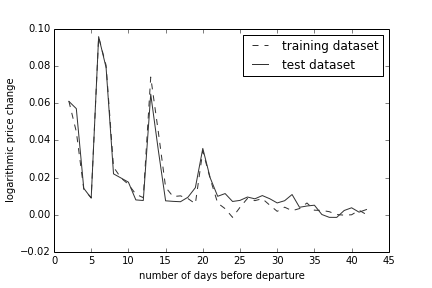
\includegraphics[width=.8\textwidth]{figures/Train-Test_DailyReturns}
\caption{Daily price changes of both datasets}
\label{fig:DailyPriceChangesBothSets}
\end{figure*}


As stated before, the difference amongst the two datasets is expected to cause high forecasting errors in the practically implementable simulation models. However, the means of the daily price fluctuations seem to overlap as shown in the graph. Because this research is more based upon the means of a lot of observations rather than every single flight, the statistical difference of the two samples could have minimal impact on the final results.

